%!TEX program = xelatex
%!TEX output_directory = out
%!TEX jobname = Thesis Draft (22107 and 22584)
\documentclass[a4paper,11pt]{article}

\usepackage[a4paper,margin=3.5cm,top=3cm,bottom=3cm,footskip=1.5cm]{geometry}

% Import most packages and options
\usepackage{article-style}

% Language and bib options
\DeclareLanguageMapping{american}{american-apa}
\addbibresource{bibliography.bib}
\defbibheading{bibliography}[\refname]{\section*{#1}}

\setmainfont{Minion Pro}

% Title and author and date
\title{Risk analysis of classic and modern value: \\A copula approach}
\author{
  \begin{tabular}[t]{@{}c@{}}
    Gustaf Soldan\\
    {\href{mailto:22107@student.hhs.se}{22107@student.hhs.se}}
  \end{tabular}
  \hskip 1em
  \begin{tabular}[t]{@{}c@{}}
    Victor Andrée\\
    {\href{mailto:22584@student.hhs.se}{22584@student.hhs.se}}
  \end{tabular}
}
\date{\textsc{Draft 1: "Game ball"} \\
October 16, 2016}

% Main document pasted from other files
\begin{document}
\maketitle
\begin{abstract}
Lorem ipsum dolor sit amet, consectetur adipiscing elit, sed do eiusmod tempor incididunt ut labore et dolore magna aliqua. Ut enim ad minim veniam, quis nostrud exercitation ullamco laboris nisi ut aliquip ex ea commodo consequat. Duis aute irure dolor in reprehenderit in voluptate velit esse cillum dolore eu fugiat nulla pariatur. Excepteur sint occaecat cupidatat non proident, sunt in culpa qui officia deserunt mollit anim id est laborum.
\end{abstract}
\pagebreak
%!TEX root = ../main.tex
\section{Introduction}
\textcite{FF2015} find that the value factor, HML, is redundant in a four-factor model including profitability (RMW) and investment (CMA), as it has no explanatory power on monthly returns in a US 1963–2010 sample. This could mean that the classic value factor is an inferior proxy for what truly comprises value. This paper takes a risk perspective on factor equity strategies and investigates what role HML has in factor investing, given the discovery of RMW and CMA. 

How can it be that HML is subsumed by CMA and RMW? [While most factor pairs exhibit relatively low correlation, the CMA and HML pair stands out with an unconditional correlation in our sample period of approx. 0.60, indicating a much higher similarity between these two factors. For a factor pair that has this high correlation coefficient, we believe that it is important to analyze whether they are both neccessary in a portfolio, regardless of whether they add alpha or not. Furthermore, HML is value minus growth and CMA is asset reduction minus asset growth. Naturally, there could be a connection between the growth valuation component in HML and the asset growth component of CMA, and it is not surprising that there is some overlap in the component stocks [what does previous research. We therefore give extra weight to analysis on how CMA and HML relates to eachother and to a factor portfolio as a whole.]

While analyses could be made on sample data alone, we wish to thoroughly examine factors by building a conditional model of return series, that can incorporate dependencies that are otherwise hard to capture in sample data, such as time-varying correlations and tail dependence. Tail dependence is the notion that there might be significantly different dependence patterns when returns simultaneously realize in the lower or upper tail, as opposed to close to the center of the distribution. From previous research on factors~\autocite{ChristoffersenLanglois2013}, we have reason to believe that the factor strategies exhibit both tail dependence and dynamic correlations, and show that this is the case also for RMW and CMA.

Recently, copula models have attracted considerable attention in the risk management field, as they offer a numerically feasible and flexible way of estimating joint probability distributions. From a copula model, we are able to simulate one-week ahead conditional forecasts of the return series. More specifically, a copula model can be estimated with univariate models as a starting point. First, we examine the factor return series on a univariate level and find evidence of autocorrelation and volatility clustering, in line with stylized facts on financial return series, and specify univariate models from the ARMA-GARCH family to capture these dynamics. The ARMA-GARCH models achieve white noise residuals for each factor, but we show that there is still substantial dependence between the residual series, indicating multivariate dependence. The copula then uses the residual series from these models and tries to explain the interdependence. The main advantage of using a copula is that it is flexible enough to generate tail dependence as well as dynamic correlations, and might improve on the description of return series.

We revisit the regressions of \textcite{FF2015} that show a zero alpha of including HML in a four-factor portfolio of Mkt-RF, SMB, RMW and CMA, but replace monthly data with weekly data and include the momentum factor. Weekly data gives a more granular understanding of risk, as shocks are more smoothed on a monthly basis. Momentum is also included, as it is frequently used in factor equity investing.\footnote{See i.a. \textcite{Pedersen2015}, \textcite{Ilmanen2011}} 

We then test the conjecture in \textcite{FF2015} that the insignificant alpha of adding HML to a four-factor portfolio implies that a mean-variance investor should in fact not include HML in her portfolio. By saving a third of the data for out-of-sample analysis, we re-estimate the copula model and construct mean-variance optimal portfolios and study the optimal weights over time. In the mean-variance analysis, we can also quantify the Sharpe ratios of portfolios including and excluding HML and CMA respectively. In addition to Sharpe ratios, we quantify higher moment risk measures of competing portfolios, including skewness and maximum drawdown. Furthermore, the out-of-sample investing investigates the performance of different copula specifications. Do conditional and asymmetric models improve the Sharpe ratio? And what happens to other risk measures?

Finally, we study the diversification benefits of HML, RMW and CMA respectively, based on simulations from a model of joint returns. More specifically, we take the copula model of factor returns as given and investigate how close the expected shortfall of a factor portfolio can come to the theoretical optimum, which is the same portfolio's Value-at-Risk. This statistic, the conditional diversification benefit (CDB) is due to \textcite{ChristoffersenErrunzaJacobLanglois2012}, and can, in the model setting, shed light on the relative benefits of including one of the similar factors HML or CMA, respectively.

___

Tease a little results
 
___

The structure of this thesis is as follows: in \autoref{sec:2} we provide a brief literature review of factor strategies and the work on copulas relating to factors. In \autoref{sec:3} we present the data used and detail the construction of factors. In \autoref{sec:4} we present the main empirical analysis by interleaving method and results. In \autoref{sec:5} we summarize our findings and discuss their wider implications.
\pagebreak
%!TEX root = ../main.tex
\section{Literature review}
\label{sec:literature}
\textcite{FF2015} introduce two additional factors to complement the \textcite{FamaFrench1993} three-factor asset pricing model. In what is referred to as the five-factor model, the traditional factors (market, value and size) are complemented by a profitability factor and an investment factor. Both factors represent zero-cost portfolios: the profitability factor, denoted RMW (robust-minus-weak), is long firms with high operating profitability and short firms with low operating profitability, and the investment factor, denoted CMA (conservative-minus-aggressive), is long firms with low investment rate and short firms with high investment rate. The five-factor model is found to be a siginificant improvement over the three-factor model, and the two new factors appear to have made the value factor, HML (high-minus-low), redundant. More specifically, the authors show that there is no significant intercept in regressions of HML on the remaining four factors, while each of the other factors have significant intercepts in similar regressions. The high average return of the HML factor appears to be fully explained by the remaining four factors. In an investment context, this can be interpreted as the HML factor adding no alpha to a portfolio holding the remaining four factors.

\textcite{Asness2015} challenge the notion that the value factor is subsumed by the addition of investment and profitability. In their study, they add a momentum factor, as well as an enhanced HML factor, and resurrect the alpha of the value factor. This leads us to believe that momentum could play an important role in recognizing the effect of HML. The momentum factor was originally studied by \textcite{JegadeeshTitman1993} and has since been shown to be present in many financial return series~\autocite{AsnessMoskovitzPedersen2013}.

It is debated whether factor strategies constitute rational risk premia or whether they are the consequences of market imperfections and irrational behavior. There are some appealing rational stories for the return premium of HML. \textcite{FamaFrench1993} show that the HML factor is related to systematic patterns of profitability and growth, and could proxy for a common risk source. This is supported by \textcite{LiewVassalou2000}, who show that the value factor can predict real GDP growth on data in several markets. \textcite{Zhang2005} uses a neoclassical model with rational expectations and competitive equilibrium to show that value firms have more tangible assets and are burdened by industry over-capacity in downturns, leading to higher down-market betas. \textcite{PetkovaZhang2005} find that the conditional betas of value stocks covary positively with the expected market risk premium.

Despite there being a number of rational theories, they all predict effects that are fairly small and cannot fully motivate the value premium. So far, the most pervasive explanations of the value premium are based on market imperfections and irrational behavior.\footnote{See i.a. \textcite{Ilmanen2011}}

\textcite{LakonishokShleiferVishny1994} argue that the value factor is driven by investors' overreaction to changes in earnings. They show that value firms have often experieced a decline in earnings over the last three years, lowering their book to market ratio. When earnings have gone down, investors as a group extrapolate the trend into the future and push prices away from fundamentals, giving rise to higher average returns for value firms and vice versa. Similar to \textcite{LakonishokShleiferVishny1994}, \textcite{BarberisHuang2001} draw on the fact that value firms have experienced decreasing earnings, but suggest that the premium is driven by investors' loss aversion bias. Current value firms have had falling earnings, leading to lower share prices and negative returns. As investors are deterred by the past performance of negative returns in itself, they are less willing to hold value stocks. \textcite{LakonishokShleiferVishny1992} instead find an explanation in the structure of the money manager industry. They suggest that there money managers have career based incentives to avoid value stocks as such stocks are more likely to go bankrupt, and make the short-term performance look bad, than growth stocks, which are more widely held in the reference index.

Variations of the long-short strategy of the value factor has become a staple strategy of both quantitative and qualitative hedge funds, often under the "equity market neutral" or "fundamental quantitative" labels. Factor equity strategies have also become increasingly accessible for retail investors, especially with the advent of smart beta ETFs. \footnote{See i.a. \textcite{Pedersen2015}, \textcite{AQREMN} and \textcite{McKEMN}.} 

The use of leverage in hedge funds can exacerbate the flow patterns in factor strategies, as highlighted by the quant crash in July-August 2007. \textcite{KhandaniLo2011} and \textcite{KhandaniLo2007} revisit the sudden and large losses of factor strategies (including value and size) during this period, and provide evidence for the "Unwind hypothesis": The crash started with rapid sell-offs of large blocks of factor strategy portfolios, for which there was not enough liquidity to maintain prices. The price drops, in turn, led to further liquidations due to 1) margin calls in other leveraged and long-short funds and 2) risk management policies, even in traditional long-only funds. This liquidity and margin spiral is very similar to that proposed by \textcite{Brunnermeier2009} and \textcite{BrunnermeierPedersen2009}.

Other papers have also highlighted the risk of "crowded trades" where leverage is applied. \textcite{Stein2009} shows that markets can become less pricing efficient and have increased chances of large fire-sale crashes when rational investors set their leverage level unknowing of how many others are engaging in a similar trade. \textcite{LouPolk2013} introduce measures of arbitrage activity and show that momentum strategies become destabilizing and prone to crash in times of high activity. For the value strategy, high arbitrage activity is instead shown to forecast positive value returns. 

The profitability and investment factors have only recently made their way into academic literature. \textcite{NovyMarx2013} study the return differences between firms with high and low gross profitability and shows significant abnormal returns to a profitability factor. Profitability is also shown to have approximately the same power in predicting the cross-section of stock returns as does value (book-to-market). Furthermore, the profitability strategy is negatively correlated with value, and can therefore improve the investing performance of a value strategy. \textcite{CooperGulenSchill2008} investigate investment, measured as the percentage change in total assets, and show that the related zero-cost-portfolio provides significant abnormal returns and that it has additional predictive ability in the cross-section of stock returns, taking both value and size into account.

While all other factor pairs are nearly uncorrelated or negatively correlated, the value (HML) and investment (CMA) factors are highly positively correlated. \textcite{Zhang2005} predicts this positive relation in a model setting, and \textcite{AndersonGarciaFeijoo2006} confirm it on empirical data. More specifically, the empirical study shows that past investment has a significant positive relation with the book-to-market ratio. In other words, value firms with high book-to-market might be value firms precisely because they have invested little, and vice versa. \textcite{FF2015} consider it a fact that value firms invest less than growth firms.

There are only a handful of papers that study factor strategies using copula methods. A working paper by \textcite{CholleteNing2012} examine dynamic correlations between a four-factor model and aggregate US consumption, and find evidence for tail dependence across the five risk factors. \textcite{ChristoffersenLanglois2013} study the four-factor model alone on US data 1963-2010, and show significant and asymmetric tail dependence that cannot be captured by standard linear correlation measures. A skewed Student-\textit{t} copula-GARCH model is found to be able to generate the model fairly well, and the authors proceed with 20 years of out-of-sample analysis on investing based on conditional expectations from the copula model, leading to significant improvements for investors with a CRRA utility function. To the best of our knowledge, no paper has previously studied the role of the investment and profitability factors using copula models.
\pagebreak
%!TEX root = ../main.tex
\section{Method}
\subsection{Getting to know the data: Diagnostic plots of marginal return series}

\subsection{Univariate ARMA-GARCH modeling of factor return series}

\subsection{Rolling correlations}
We compute rolling correlation estimates in order to investigate whether the factor equity strategies exhibit constant correlation over time. 
\begin{align}
    RCorr(r_{i, t}, r_{j, t})_t^{w} = \frac{\sum^{t}_{t-w+1}(r_{i, t} - \bar{r}_i)(r_{j,t} - \bar{r}_j)}{\sqrt{\sum^{t}_{t-w+1} (r_{i,t} - \bar{r}_i)^2} \sqrt{\sum^{t}_{t-w+1} (r_{j,t} - \bar{r}_j)^2}}
\end{align}
where $r_i$, $r_j$ are the $N \cdot (N-1) / 2$ different pairs of the factor strategies' log returns and $w$ is the rolling window of data. We use approximately one year of data with $w = 45$ on weekly data.
\subsection{Threshold correlations}
Threshold (or exceedance) correlations have previously been used to highlight the tail dependence of i.a. country equity indices~\autocite{LonginSolnik2001}, portfolios by industry, size, value and momentum~\autocite{AngChen2002} and factor strategies~\autocite{ChristoffersenLanglois2013}. However, no paper has previously studied threshold correlation between factors when including the RMW and CMA factors. We follow~\textcite{ChristoffersenLanglois2013} definition of threshold correlation
\begin{align}
    TCorr(r_i, r_j) = 
    \begin{cases} 
        Corr\Big(r_i, r_j \,|\, r_i < F_i^{-1}(p), r_j < F_j^{-1}(p)\Big)  & \text{for } p < 0.5 \\
        Corr\Big(r_i, r_j \,|\, r_i \geq F_i^{-1}(p), r_j \geq F_j^{-1}(p)\Big)  & \text{for } p \geq 0.5
    \end{cases}
\end{align}
where $F_i^{-1}(p)$ the empirical quantile of $r_i$ at percentile $p$. Graphically, threshold correlation can be understood from \autoref{diag:thresholdexplain}. 
\begin{figure}[H]
  \caption{Threshold correlation - conceptual plot}
  \label{diag:thresholdexplain}
  %\toprule
  \centering
  \begin{minipage}{\textwidth}
  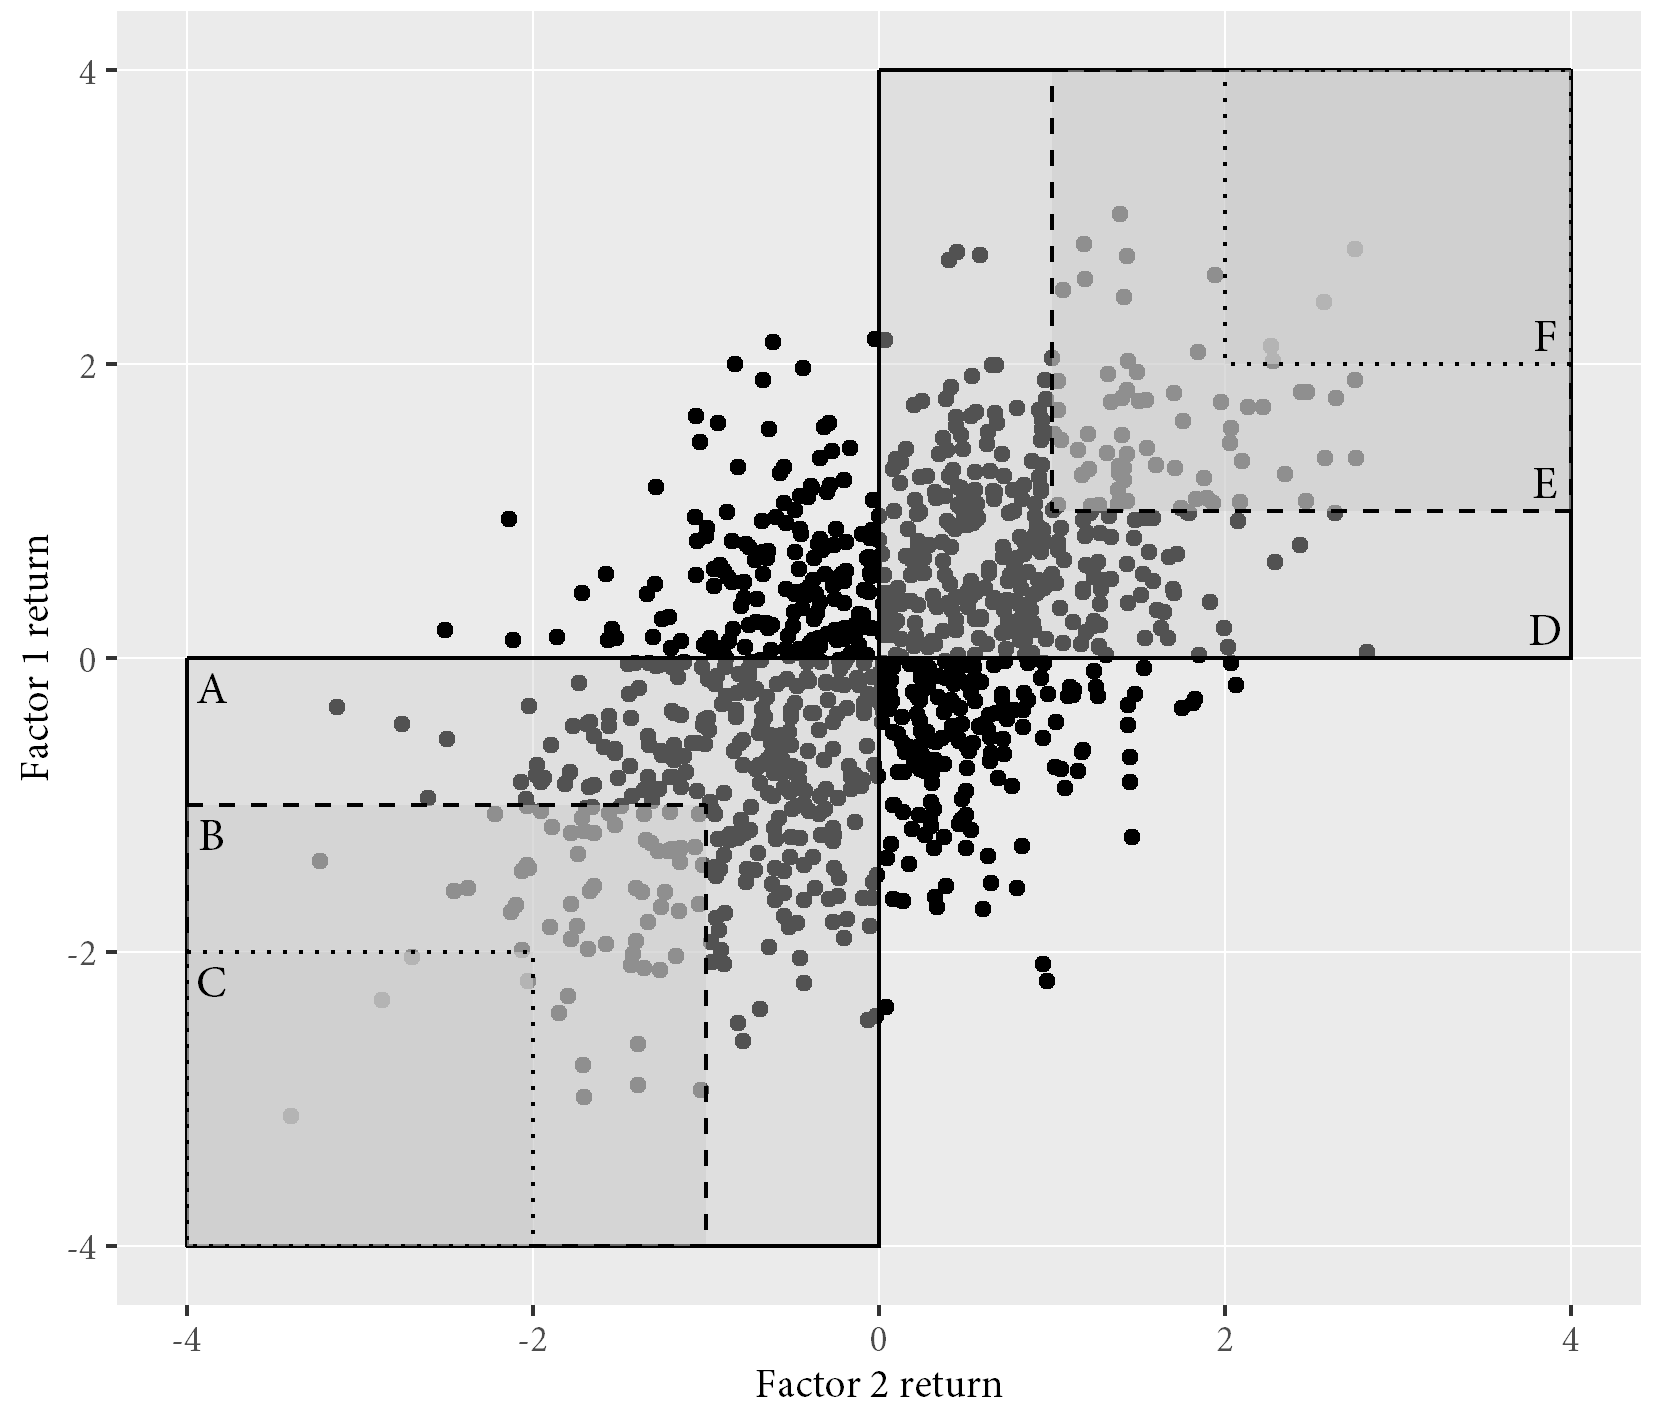
\includegraphics[scale=1]{graphics/threshold_explain.png}  
  %\bottomrule
  \vspace{3mm}
  \footnotesize
  Conceptual plot of threshold correlations coefficients. A, B and C areas represent threshold correlation subset of data when $p<0.50$ and D, E and F areas represent subsets when $p\geq0.50$. The data is a random generation of 1,000 observations from a bivariate standard normal distribution with correlation coefficient 0.5.
  \end{minipage}
\end{figure}
For $p = 0.49$, the first value below the median, threshold correlation is the linear correlation in the subset of data that is in area A. As $p$ approaches zero, the area A becomes smaller and smaller, illustrated by B and C. Above the median, the same is illustrated by areas D, E and F. Ceteris paribus, assets pairs with weaker or negative threshold correlation as $p < 0.50$ are better diversified, as they tend to coincide in extreme negative returns less often. Although threshold correlations are simply the linear correlations for a subset of the data, they do give a measure of tail dependency - how correlated are returns when times are extreme? Furthermore, they provide an indirect way of testing whether variables are jointly normal distributed, as the threshold correlation of normally distributed variables tends to zero as $p$ approaches zero or one. For jointly Student-\textit{t} distributed variables, this is not the case, and for jointly skewed Student-\textit{t} distributed variables, threshold correlations can also be asymmetric, i.e. different above and below the median.
\subsection{Copula}
Copulae provide a numerically feasible way to estimate a multivariate distribution function, which can then be used to draw inferences and simulate return series.~\textcite{Patton2006} uses the theorem of~\textcite{Sklar1959} to show that the conditional multivariate distribution function of log returns can be decomposed into a copula function and the product of univariate distributions
\begin{align} \label{eq:sklar}
    f_t(r_{1,t+1}, ..., r_{N, t+1}) &= c_t(u_{1, t+1}, ... u_{N, t+1}) \prod^N_{i=1} f_{i,t}(r_{i, t+1})
\end{align}
where $c_t(u_{1, t+1}, ... u_{N, t+1})$ is the copula density function, in this application taking uniform transformations of residuals from the ARMA-GARCH model, $\{u_i\}$, as arguments. This relies on a two-step maximum likelihood procedure (also known as the inference-by-margins (IFM) procedure) introduced by~\textcite{Joe1997}, which starts by estimating with the marginal distributions and subsequently estimates the copula function, using the margin residuals as given. For details on the marginal estimation procedure, see \autoref{App:AppendixB} The IFM method drastically improves the speed of the optimization process in large data sets; however, it is not efficient as shown by~\textcite{ChenFanTsyrennikov2006}, who instead propose a sieve ML estimation. This paper still employs IFM, as the efficiency loss is small in most cases~\autocite{Patton2006}. 

We focus on a skewed Student-\textit{t} copula, parameterized by $\Theta = \{\nu, \gamma, R\}$ using the constant correlation specification, and by $\Theta^{cDCC} = \{\nu, \gamma, \alpha, \beta, R\}$ using the dynamic correlation process. The analysis closely follows in the footsteps of~\textcite{Aielli2013} and~\textcite{ChristoffersenErrunzaJacobLanglois2012}. The skewed Student-\textit{t} distribution is described in detail in \autoref{App:AppendixA}.

The normal and Student-\textit{t} copulas are both nested in the skewed Student-\textit{t} model, as the degree of freedom and skewness parameters go to infinity and zero respectively. Results are presented for all three copulas, with and without correlation dynamics. The model selection criteria is BIC (\textcite{Schwarz1978}).

\textbf{Constant correlation specification}

As a benchmark model, we consider the case of a constant correlation matrix between the factor strategies' ARMA-GJR-GARCH residuals. 

The copula parameters $\Theta = \{\nu, \gamma, R_t\}$ are estimated using ML of the copula function, where $\nu$ is the degree of freedom, $\gamma$ is the vector of skewness parameters and $R$ is the constant copula correlation matrix. Rearranging Sklar's Theorem in \autoref{eq:sklar} and taking logs, the copula log-likelihood function is
\begin{align} \label{eq:constantllf}
    LLF(\nu, \gamma, R; u_1, ..., u_T) = \sum^T_{t=1} \Big \{ ln f_t(\varepsilon_{t}; \nu, \gamma, R) - \sum^N_{i = 1} ln f_{i,t}(\varepsilon_{i, t}; \nu, \gamma) \Big \}
\end{align}
where the density function $f$ is the skewed Student-\textit{t} given by \autoref{eq:dskewt}.

\textbf{\textit{c}DCC conditional correlation process}

To capture time-varying dependency, as motivated by rolling correlation and threshold correlation analyses, the copula correlation matrix $R_t$ is allowed to vary over time according to the \textit{c}DCC model~\autocite{Aielli2013}\footnote{\textit{c} stands for corrected, as Aielli (2009) has shown that the standard DCC estimator of Engle (2002) and Tse \& Tsui (2002) can be inconsistent.}
\begin{align} \label{eq:qtrtlink}
    R_t &= Q_t^{-1/2} Q_t Q_t^{-1/2}
    \intertext{where the core process is}
    Q_t &= (1 - \alpha - \beta) S + \alpha z_{t-1} z_{t-1}^\top + \beta Q_{t-1} \label{eq:qprocess}
\end{align}
The $Q_t$ process is comprised of three components that are weighted according to $\alpha, \beta$: (1) $S$, a time-invariant component, to be interpreted similarly to a long-term mean in a regular GARCH process as $\mathbb{E}[Q_t] = S$, (2) $z_{t-1} z_{t-1}^\top$, an innovation component from the copula shocks, and (3) $Q_{t-1}$, an autoregressive component of order one. In order for the the correlation matrix $R_t$ to be positive definite, $Q_t$ has to be positive definite, which is ascertained by requiring that $\alpha \geq 0$, $\beta \geq 0$ and $(\alpha + \beta) < 1$.

The parameters $\alpha, \beta$ are simultaneously estimated with the skewed Student-\textit{t} parameters $\nu$ and $\gamma$ using ML for the copula function, whose log-likelihood function is again found by rearranging Sklar's theorem (\autoref{eq:sklar}) and taking logs on both sides
\begin{align} \label{eq:cdccllf}
    LLF(\nu, \gamma, \alpha, \beta, R_t; u_1, ..., u_T) = \sum^T_{t=1} \Big \{ ln f_t(\varepsilon_{t}; \nu, \gamma, \alpha, \beta, R_t) - \sum^N_{i = 1} ln f_{i,t}(\varepsilon_{i, t}; \nu, \gamma) \Big \}
\end{align}
where the density function $f$ is the skewed Student-\textit{t} given by \autoref{eq:dskewt}.

The process of the copula estimation with \textit{c}DCC dynamics is quite involved, as it relies on moment matching and recursive estimation of parameters to estimate the copula correlation matrices $\{\hat{R_t}\}$. See \autoref{App:AppendixD} for a detailed description.

\textbf{Extending the cDCC model with exogenous regressors}

\Textcite{ChristoffersenErrunzaJacobLanglois2012} consider an extension of~\eqref{eq:qprocess}, where the long-running component $S$ is extended with a time-varying component in a general manner. Replace $S$ with a weighted average of a time-invariant component $\Omega$ and a time-varying component $\Upsilon_t$, to get:
\begin{align}
    S_t &= (1 - \phi) \Omega + \phi \Upsilon_t
\end{align}
$\Upsilon_t$ can support any number of common or factor-specific regressors, such as a common time-trend, conditional volatilities or arbitrage activity. We detail how we construct it in~\autoref{App:AppendixD}.

\begin{quote}
    \textit{Draft Note:} Using $\Upsilon_t$ we will be able to model how the dynamics of tail-dependency change with arbitrage activity, which relates to the second/extended parts of our paper. We have yet to get ahold of the data necessary to estimate this model. For practical purposes, we are looking to move forward with just one copula distribution (likely symmetric Student's t since the asymmetries don't appear that great).

    At its most simple, we can use a simple time trend as in~\autocite{ChristoffersenErrunzaJacobLanglois2012}. However, we would like to use data from Lipper, for which we don't have access yet.
\end{quote}

\textbf{Copula-based expected shortfall}

By simulating many runs of one-week-ahead copula shocks, we can find the simulated probability distributions for one-week-ahead factor strategy returns. The process is as follows
\begin{enumerate}[(i)]
    \item At $t = T$, generate 10,000 one-week-ahead random copula shock vectors $z_{T+1}$ according to the conditional copula correlation matrix $\hat{R}_{T+1}$
    \item Transform each $z_{T+1}$ vector to uniform shocks using copula parameters
    \item Transform each uniform shocks vector to GARCH residuals using marginal distribution parameters
    \item Forecast the ARMA-GJR-GARCH process using the residual vectors to get the simulated return vectors $r_{T+1}$
    \item Infer the empirical distribution function of $T+1$ returns using the simulated return vectors
    \item Repeat steps (i)-(v) at $t = T+1, T+2, ...$
\end{enumerate}
The VaR and ES are then found by
\begin{align}
    VaR_{i,T+1}^{1-\alpha} &= F_{i, T+1}^{-1}(\alpha | I^{sim}_T) \\
    ES_{i, T+1}^{1 - \alpha} &= E_t[r_{i,T+1} | r_{i,T+1} < VaR_{i,T+1}^{1-\alpha}]
\end{align}
where $F_{i, T+1}^{-1}(\alpha | I^{sim}_T)$ is the inverse empirical CDF (based on simulated data set $I^{sim}_t$) of asset $i$ at time $T+1$.

\subsection{Conditional diversification benefits}
As the copula has time-varying dependece, it must also have time-varying diversification benefits. We use a measure of conditional diversification benefits from \textcite{ChristoffersenErrunzaJacobLanglois2012} to determine how modern and classic value differ in terms of diversification benefits. 

The method is based on time-varying expected shortfall, expressed in percentage terms as
\begin{align}
    ES^p_{i,t}(r_{i,t}) = -\mathbb{E}_{t-1}[r_{i,t} | r_{i,t} \leq F_{i,t}^{-1}(p)]
\end{align}
where $r_{i,t}$ are simple returns of assets $i$ (to ensure that the weighted average return property of a portfolio holds) and $F_{i,t}^{-1}(p)$ is the conditional inverse CDF of returns for the $p\%$ quantile, which is also equivalent to the negative estimate of $p\%$ Value-at-Risk (VaR).

For the portfolio setting, return and expected shortfall are denoted as
\begin{align}
    R_{t} = \sum\limits^N_{i=1} w_{i,t} r_{i,t} \\
    ES^p_t(w_t) = -\mathbb{E}_{t-1}[R_{t} | R_{t} \leq F_{t}^{-1}(p)]
\end{align}
where $w_{i,t}$ are the dynamic portfolio weights and $F_{t}^{-1}(p)$ is the inverse CDF of the portfolio return $R$ at the $p\%$ quantile.

Unlike Value-at-Risk, expected shortfall is a coherent risk measure that is sub-additive across assets. Therefore, the combined risk measure of a portfolio is always smaller than or equal to the sum of the marginal risk measures.
\begin{align} \label{eq:es1}
    ES^p_t(w_t) \leq \sum\limits^N_{i=1} w_{i,t} ES^p_t(r_{i,t}) && \forall w_t \in \mathbb{R}
\end{align}
where $w_{i,t}$ are the dynamic portfolio weights. From the equality in \autoref{eq:es1}, we know that a upper bound on $ES$ is
\begin{align}
    \overline{ES}^p_t(w_t) = \sum\limits^N_{i=1} w_{i,t} ES^p_t(R_{i,t})
\end{align}
This corresponds to the case of zero diversification benefits. Similarly, a lower bound on the portfolio's $ES$ is
\begin{align}
    \underline{ES}^p_t(w_t) = -F^{-1}_t(w_t, p) 
\end{align}
where $F^-1_t(w_t, q)$ is the inverse CDF at time $t$ for the portfolio return with weights $w_t$. The lower bound is, in other words, equivalent to the case when the portfolio's $ES$ is equivalent to the portfolio's $VaR$.

The conditional diversification benefit statistic is now defined as
\begin{align}
    CDB_t(w_t,p) = \frac{\overline{ES}^p_t(w_t) - ES^p_t(w_t)}{\overline{ES}^p_t(w_t) - \underline{ES}^p_t(w_t)}
\end{align}

The intuition behind the statistic is best understood by focusing on the second term of the numerator and the denominator: when diversification benefits are high, the expected shortfall of a portfolio is relatively close to the Value-at-Risk, which makes the ratio close to one. When diversification benefits are poor, the expected shortfall is hardly different from the weighted average of individual expected shortfalls, and the ratio is close to zero.

The statistic is dependent on the calculation of $ES^p_t(w_t)$ which can only be found by simulation. In line with \textcite{ChristoffersenErrunzaJacobLanglois2012}, we maximize $CDB_t(w_t,p)$ at each time $t$ by simulating 10,000 draws of 1-week-ahead returns, using the skewed Student-\textit{t} copula model with \textit{c}DCC correlation dynamics. This yields a series of optimal $\{CDB^*\}$ for corresponding optimal dynamic weights $\{w^*_t\}$.

In the empirical results, we report three different graphs of $CDB^*$ when $p=5\%$, with different restrictions on portfolio weights in the optimization: In the first, three portfolios are available, one with all six factor strategies, one with classic value (all, but excluding RMW, CMA) and one with modern value (all, but excluding HML). In the second, two portfolios are available, one with all factors excluding HML, and one with all factors excluding CMA. This graph is meant to disentangle the risk of HML and CMA respectively. In the third, three portfolios are available, one with Mkt.RF, HML, SMB and Mom, one with Mkt.RF, SMB, Mom and CMA, and one with Mkt.RF, SMB, Mom and RMW. This graph is meant to look at the three value factors marginal contributions.

There are also two general restrictions on the portfolios: First, all factor weights must be positive, as the interpretation of a negative factor weight is the same as betting against the factor. Note that this does not mean that short sales are prohibited, as factor strategies are inherently long-short. Second, factor weights must sum to 1, as we do not consider the case of leverage.

\subsection{Mean-variance investing}
As the classic value factor is shown to add no alpha to a portfolio of the remaining four factors in the five-factor model \autocite{FF2015}, we examine the impact of excluding HML from the investible universe.

By simulating 10,000 draws of 1-week-ahead returns, using the skewed Student-\textit{t} copula model with \textit{c}DCC correlation dynamics, we can estimate the conditional expected return vector and variance-covariance matrix. This allows us to conduct mean-variance investing based on estimates from the copula model. As previously, we impose the two general restrictions that all factor weights must be positive, and that factor weights must sum to 1, which makes the tangency portfolio without a risk-free asset the optimal portfolio. At the end of each week $t$, the optimization problem becomes
\begin{align}
    \max_{w} w^\top \mu - \frac{\gamma}{2}\,w^\top \Sigma w && s.t. w^\top \mathbf{1}_N = 1
\end{align}
where $w$ is the set of weights, $\mu$ is the expected return, $\gamma$ is the risk aversion, $\Sigma$ is the variance-covariance matrix, and $\mathbf{1}_N$ is a vector of ones. The tangency portfolio solution is
\begin{align}
    w^* = \frac{1}{\mu^\top \Sigma^{-1} \mathbf{1}_N} \, \Sigma^{-1} \mu
\end{align}
In parallel, we consider two investible asset universes, one with all six factor strategies and one without HML. We then consider the impact of excluding HML on a number of realized performance measures including: Sharpe ratio, maximum drawdown and skewness. [The hypothesis is that there will only be a minor impact on the Sharpe ratio, while maximum drawdown and skewness improve]

\pagebreak
%!TEX root = ../main.tex
\subsection{Copula specification and estimation results}
Given the results of the dependence structure of residuals, we now discuss the best choice of copula model and present estimation results of the six competing copula specifications.

We have estimated constant and dynamic normal, symmetric \emph{t} and skewed \emph{t} copula models on the full dataset of uniform GARCH residuals. Results are presented in~\autoref{tab:copula_estimation}. 

First, we examine the choice between a normal, symmetric \emph{t} or skewed \emph{t} copula. We note that $\nu_c$ is clearly significant and suggests one of the Student's \emph{t} models with tail dependence over the normal model. Second, we examine the asymmetric specification and find that few of the $\gamma_c$ estimates appear significant. This indicates that the asymmetry is hard to capture, or that it is not well represented by this type of model. This is supported by the relatively small improvement in log-likelihood in going from a symmetric \emph{t} to skewed \emph{t} copula, and also by the fact that the BIC criterion prefers the symmetric \emph{t} model in the dynamic case. 

Second, we examine the choice between a constant and dynamic copula correlation matrix. There is a significant improvement in log-likelihood and BIC when moving from a constant to a dynamic copula, which suggests that time-varying dependence shown by rolling correlation is captured and improves the model's fit. We also find a high persistence of the correlation process, as $\alpha + \beta$, is close to a unit root.

In summary, we find that the dynamic symmetric \emph{t} copula is the best specification, as it has the lowest BIC, well defined parameters, and is strongly supported by the dependence pattern showcased by threshold and rolling correlation analyses. While the skewed \emph{t} copula is an interesting model, we believe that the asymmetry patterns in data are too irregular to be well captured by a copula model with only one asymmetry parameter for each series (this is further discussed in the subsequent robustness discussion, see \autoref{sub:05_robust}).

%!TEX root = ../../main.tex

\begin{table}[!ht]
  \centering
  \scriptsize
  \renewcommand{\arraystretch}{1.2}

  \caption{Parameter estimates for copula models based on uniform residuals from ARMA-GJR-GARCH models.\\ \quad \\
  Stationary bootstrap standard errors in parentheses, following Politis and Romano (1994). Copula parameters: $\nu_c$ is the degree of freedom, $\gamma_c$ is the vector of skewness parameters, $\alpha$, $\beta$ are the shock loading and autoregressive loading of the cDCC process. The significance test of $\nu_c$ is based on $1/\nu_c$, as this ratio goes to zero when $\nu_c$ goes to infinity (normality). Sample: 1963-07-05--2016-07-01.}
  \begin{tabularx}{\textwidth}{@{}l ddd X ddd @{}}
    \toprule
    &
      \multicolumn{3}{c}{Constant Copula} &&
      \multicolumn{3}{c}{Dymamic Copula} \\
    \cmidrule{2-4} \cmidrule{6-8}
    &
      \multicolumn{1}{c}{Normal} & \multicolumn{1}{c}{Symmetric \emph{t}} & \multicolumn{1}{c}{Skewed \emph{t}} & &
      \multicolumn{1}{c}{Normal} & \multicolumn{1}{c}{Symmetric \emph{t}} & \multicolumn{1}{c}{Skewed \emph{t}} \\
    \midrule
    $\nu_c$ & & 6.625^{**} & 6.671^{**} && & 11.936^{**} & 11.881^{**} \\
    & & (0.636) & (0.264) && & (0.770) & (0.641) \\
    \\
    $\gamma_\text{Mkt}$ & & & -0.057 && & & -0.078 \\
    & & & (0.047) && & & (0.062) \\
    \\
    $\gamma_\text{HML}$ & & & 0.103 && & & 0.083 \\
    & & & (0.036) && & & (0.071) \\
    \\
    $\gamma_\text{SMB}$ & & & -0.103 && & & -0.175 \\
    & & & (0.055) && & & (0.098) \\
    \\
    $\gamma_\text{Mom}$ & & & -0.202^{**} && & & -0.145 \\
    & & & (0.032) && & & (0.073) \\
    \\
    $\gamma_\text{RMW}$ & & & 0.021 && & & 0.095 \\
    & & & (0.035) && & & (0.058) \\
    \\
    $\gamma_\text{CMA}$ & & & 0.076 && & & 0.001 \\
    & & & (0.038) && & & (0.050) \\
    \\
    $\alpha$ & & & && 0.065 & 0.068^{**} & 0.068^{**} \\
    & & & && (0.006) & (0.006) & (0.006) \\
    \\
    $\beta$ & & & && 0.915 & 0.913^{**} & 0.913^{**} \\
    & & & && (0.008) & (0.007) & (0.007) \\
    \midrule
    Log-likelihood & 1169.194 & 1555.683 & 1572.672 && 2790.618 & 2977.648 & 2989.273 \\
    No. of Parameters & 15 & 16 & 22 && 17 & 18 & 24 \\
    % BIC & -348.32 & -122.21 & -316.432 && -243.221 & -342.342 & -396.324 \\
    Persistence & & & && 0.981 & 0.981 & 0.981 \\
    \bottomrule
  \end{tabularx}

  \label{tab:copula_estimation}
\end{table}

\pagebreak
%!TEX root = ../main.tex
\appendix
\appendixpageoff
\section{Appendix A. Skewed Student-\textit{t} distribution} \label{App:AppendixA}
In line with stylized facts on financial return series, the factor strategies exhibit fat tails and skewness - features that are poorly represented by the normal Gaussian. Our univariate estimations as well as our copula builds on the~\textcite{Hansen1994} skewed Student-\textit{t} distribution. The skewed Student-\textit{t} distribution is, more generally, nested in the generalized hyperbolic distribution~\autocite{McNeilFreyEmbrecht2005}.

The random vector X is distributed multivariate generalized hyperbolic if
\begin{align}
    X \sim \mu + \sqrt{W} A Z + \gamma W
\end{align}
where $\mu$ is the location vector, $\gamma$ is the skewness vector, $R = A A^\top$ is the dispersion matrix, $W$ follows a generalized inverse-gamma distribution $W \sim GIG(\lambda, \chi, \psi)$ and Z is multivariate normal $Z \sim N(\mu^N, R)$, with $W, Z$ independent. The skewed Student-\textit{t} is nested with parameters
\begin{align}
    \lambda = \frac{\nu}{-2} && \chi = \nu - 2 && \psi = 0
\end{align}
where $\nu$ is the degree of freedom. Furthermore
\begin{align}
    \mathbb{E}[X] &= \mu + \mathbb{E}[W] \gamma \\
    Var[X] &= \mathbb{E}[Cov(X|W)] + Cov(\mathbb{E}[X|W]) \\
    &= Var(W) \gamma \gamma^\top + \mathbb{E}[W] R \nonumber
\end{align}
These moments describe the link between the copula correlation matrix $R$ and the skewed Student-\textit{t} distribution's dispersion matrix $R$. Covariances are finite when $\nu > 4$. The multivariate density function is given by
\begin{align} \label{eq:dskewt}
    f_X(x) &= \frac{(\nu - 2)^\frac{\nu}{2} (\gamma^\top R^{-1} \gamma)^{\frac{\nu+d}{2}}}{(2 \pi)^{\frac{d}{2}} |R|^\frac{1}{2} \Gamma (\frac{\nu}{2}) 2^{\frac{\nu}{2} - 1}} \cdot \frac{K_{\frac{\nu + d}{2}} ( \sqrt{(\nu - 2 + Q(x)) \gamma^\top R^{-1} \gamma}) e^{(x-\mu)^\top R^{-1} \gamma} )}{( \sqrt{(\nu - 2 + Q(x)) \gamma^\top R^{-1} \gamma})^{\frac{\nu + d}{2}}}
\end{align}
where $K(\cdot)$ is the modified Bessel function of the second kind, $Q(x) = (x-\mu)^\top R^{-1} (x-\mu)$, $d$ is the length of $x$, and $\Gamma$ is the gamma distribution density.

\newpage
\section{Appendix B. ARMA-GARCH modeling of marginal distributions} \label{App:AppendixB}

By examining marginal factor strategy returns (see \autoref{App:AppendixF}), we find evidence of non-normality, autocorrelation, volatility clustering and leverage effects, in line with stylized factors on financial return series (\textcite{Bollerslev1986}, \textcite{Black1976}, \textcite{glosten1993relation}). An ARMA-GARCH model allows us to filter away such marginal asymmetries, while leaving any multivariate asymmetry to the copula specification. 

The most important goal of this application GARCH model is not to have high predictive power of asset return series, but to sanitize the data to be used in multivariate analysis. We focus on parsimonious models with few lags, but enough flexibility to capture salient features of the summary plots of the marginal series, such as volatility clustering and leverage effect.

The selection process is as follows: for each factor strategy, ARMA-GJR-GARCH models are estimated with different ARMA lag orders (up to 3,3) and a fixed GJR-GARCH order of (1,1). We then compute the Bayesian Information Criterion (BIC, \textcite{Schwarz1978}) for each specification, and for each factor select the model with the lowest BIC as the primary candidate. The primary candidate specification is then checked for remaining serial correlation and ARCH effects in residuals, using the weighted portmanteau tests of \textcite{FisherGallagher2012}. All of the primary candidate models pass the diagnostic tests (see \autoref{App:AppendixE}), and additional diagnostics plots are available (see \autoref{App:AppendixG}). We use the GJR-GARCH model with ARMA mean equation
\begin{align}
    r_t &= \mu + \sum^p \phi_p r_{t-p} + \sum^q \theta_q \epsilon_{t-q} + \epsilon_{t}  \\
    \sigma_{t}^2 &= \omega + (a + \eta I_{t-1}) \epsilon_{t-1}^2 + b \sigma^2_{t-1}
\end{align}
which is estimted using maximum likelihood for each of the factor return series. The innovations $\epsilon_{i,t}$ are assumed to be distributed skewed Student-\textit{t} with skewness $\zeta$ and degree of freedom $\varrho$.

Using conditional one-step-ahead forecasts of log return and standard deviation from the ARMA-GARCH model, we can compute standardized GARCH residuals
\begin{align}
    \epsilon^*_{i,t} = \frac{\epsilon_{i,t} - E_{t-1}[\epsilon{i,t}]}{E_{t-1}[\sigma(\epsilon{i,t})]}
\end{align}
which are subsequently transformed into uniform residuals using the inverse of the skewed Student-\textit{t} distribution (\autoref{eq:dskewt}). The uniform series $\{u_i\}$ are then employed in the copula estimation.
\begin{align}
    u_{i,t} = t^{-1}_{\zeta, \varrho}(\epsilon^*_{i,t})
\end{align}

\newpage
\section{Appendix C. Stationary bootstrap of copula parameter standard errors} \label{App:AppendixC}
We rely on the multi-step maximum likelihood estimation of the copula model, which takes the standardized residuals of marginal distributions as given in the second step. The first estimation step introduces parameter uncertainty that is not taken into account by the conventional standard errors of the second estimation.\footnote{Here, our model deviates from~\textcite{ChristoffersenLanglois2013}, who use a semi-parametric model that uses the empirical density function, and find standard errors using the analytical approach in~\textcite{ChenFan2006}. However, those errors are not valid in a time-varying copula context, as the estimation of means and variances impact the asymptotic distributions of copula parameters~\autocite{Remillard2010}.} We use the stationary block bootstrap method of \textcite{PolitisRomano1994} with a block length of 45 weeks (approx. 1 year of data) to find reliable standard errors for copula parameters. The procedure is theoretically supported by \textcite{GonclavesWhite2004} and implemented as follows:
\begin{enumerate}[(i)]
    \item Generate a block bootstrap version of the original weekly return data
    \item Estimate the ARMA-GJR-GARCH models and calculate standardized residuals
    \item Transform standardized residuals to uniform and estimate the copula model
    \item Collect the copula parameters $\Theta_i$
    \item Repeat (i)-(iv) N times to get $\{\Theta_i\}^{N}_{i=1}$
    \item Use the standard errors from the empirical distribution of $\{\Theta_i\}^{N}_{i=1}$
\end{enumerate}

\newpage
\section{Appendix D. Copula correlation matrix estimation with \textit{c}DCC dynamics} \label{App:AppendixD}
This is a step-by-step description of the procedure used to find the copula correlation matrix $\{\hat{R_t}\}$ in the \textit{c}DCC case, and has been adapted from \textcite{Aielli2013}.
\begin{enumerate}[(i)]
    \item Re-standardize uniform residuals from univariate ARMA-GJR-GARCH models $\{u_{i}\}$ using the inverse skewed Student-\textit{t} distribution with copula parameters $\nu, \gamma$,  and scale to zero mean and unit variance using the conditional mean and standard deviation\footnote{Unless the copula is normal, the re-standardized residuals $\{\varepsilon^c_i\}$ will not have zero mean and unit variance, which is required for the estimation of the sample correlation matrix $\hat{S}$.}
    \begin{align}
        \varepsilon^c_{i,t} = t^{-1}_{\gamma, \nu}(u_{i,t})
    \end{align}
    \begin{align}
        \varepsilon_{i,t} = \frac{\varepsilon^c_{i, t} - E_{t-1}[\varepsilon^c_{i,t}]}{E_{t-1}[\sigma(\varepsilon^c_{i,t})]}
    \end{align}
    \item Compute the diagonal elements in $Q_t$ over time recursively, initializing with unit diagonal, and using Q-residuals $\{z_i\}$
    \begin{align}
        \intertext{Utilizing that $\S_{ii} = 1$ (for any correlation matrix), the process for diagonal elements of Q simplifies to}
        q_{ii, t} &= (1 - \alpha - \beta) + \alpha z_{t-1} z_{t-1}^\top + \beta q_{ii, t-1}
        \intertext{where residuals $\{z_{i}\}$ are initialized at zero and then calculated as}
        z_{i, t} &= \varepsilon_{i, t} \sqrt{q_{ii, t}}
    \end{align}
    \item Use Q-standardized residuals $\{z_{i}\}$ to calculate a copula sample correlation matrix
    \begin{align}
        \hat{S} = \frac{1}{T} \sum_{t=1}^{T} z_{t-1} z_{t-1}^\top
    \end{align}
    \item Calculate off-diagonal elements of the Q matrix using the copula sample correlation matrix $\hat{S}$ as the long-term correlation matrix in the \textit{c}DCC specification
    \begin{align}
        \hat{Q_t} = (1 - \alpha - \beta) \hat{S} + \alpha z_{t-1} z_{t-1}^\top + \beta Q_{t-1}
    \end{align}
    \item Standardize $\hat{Q_t}$ to the copula correlation matrix $\hat{R_t}$ (\autoref{eq:qtrtlink}) and calculate the sum of log-likelihoods for a given parameter set $\Theta = \{\nu, \gamma, \alpha, \beta\}$ (\autoref{eq:cdccllf})
\end{enumerate}
\newpage
\section{Appendix E. ARMA-GJR-GARCH estimation results}
\label{App:AppendixE}
% TABLES NEED TO BE MODIFIED IN THE FOLLOWING WAYS
% 1) Change {tabular} to {tabularx}{\textwidth} and make leftmost column an X column
%     and change top and bottom \hline to \toprule \bottomrule
%
% paste the following at start but before & \multicolumn
%
% \begin{tabularx}{\textwidth}{@{\extracolsep{5pt}} X D{.}{.}{-3} D{.}{.}{-3} D{.}{.}{-3} } 
% \\[-1.8ex] \midrule
% \\[-1.8ex] 
%
% paste the following at end after R2 row but before Note row
% \bottomrule \\[-1.8ex] 
%
% 2) Change the variable names to greeks
% 3) Change specification names if needed
% 4) Change R2 to LLH and add similar lines for Ljung-Box and ARCH-LM
% 5) Add label and caption
% 6) Paste this to get table heading description
%
% \begin{tabularx}{\textwidth}{X}
% \\[-1.8ex]\toprule
%\\[-1.8ex] 
% text goes here
% \end{tabularx}
%
% 6) Copy the whole table, only change caption, label, factor/spec labels and (1)-(3) to (4)-(6)
\begin{table}[!htbp] \centering 
  \caption{GARCH results: Mkt.RF, HML, SMB} 
  \label{tab:garch1} 
\begin{tabularx}{\textwidth}{X}
\\[-1.8ex]\toprule
\\[-1.8ex] 
\footnotesize Parameter estimates from ARMA-GJR-GARCH models. Heteroskedasticity robust standard errors in parentheses, following \textcite{White1982}. All data 1963-07-05 - 2016-07-01. Mean equation: $r_t = \mu + \sum^p \phi_p r_{t-p} + \sum^q \theta_q \epsilon_{t-q} + \epsilon_{t}$ and variance equation: $\sigma_{t}^2 = \omega + (a + \eta I_{t-1}) \epsilon_{t-1}^2 + b \sigma^2_{t-1}$. $\zeta, \varrho$ are the skewness and degree of freedom parameters of the Skewed Student-\textit{t} innovations. $\omega$ is set using variance targeting, following \textcite{EngleMezrich1995}. Ljung-Box and ARCH-LM tests are the weighted portmanteau tests with automatic lag selection from \textcite{FisherGallagher2012}.
\end{tabularx}
\begin{tabularx}{\textwidth}{@{\extracolsep{5pt}} X D{.}{.}{-3} D{.}{.}{-3} D{.}{.}{-3} } 
\\[-1.8ex]\midrule
\\[-1.8ex] 
 & \multicolumn{3}{c}{Factor series} \\ 
\cline{2-4} 
\\[-1.8ex] & \multicolumn{1}{c}{(1)} & \multicolumn{1}{c}{(2)} & \multicolumn{1}{c}{(3)}\\ 
\\[-1.8ex] & \multicolumn{1}{c}{Mkt.RF} & \multicolumn{1}{c}{HML} & \multicolumn{1}{c}{SMB}\\ 
\hline \\[-1.8ex] 
 $\mu$ & 0.001^{***} & 0.001^{**} & 0.000 \\ 
  & (0.000) & (0.000) & (0.000) \\ 
  & & & \\ 
 $\phi_1$ &  & 0.735^{***} & 0.779^{***} \\ 
  &  & (0.076) & (0.043) \\ 
  & & & \\ 
 $\theta_1$ &  & -0.621^{***} & -0.654^{***} \\ 
  &  & (0.085) & (0.055) \\ 
  & & & \\ 
 $a$ & 0.088^{***} & 0.109^{***} & 0.110^{***} \\ 
  & (0.012) & (0.002) & (0.024) \\ 
  & & & \\ 
 $b$ & 0.851^{***} & 0.872^{***} & 0.844^{***} \\ 
  & (0.004) & (0.002) & (0.036) \\ 
  & & & \\ 
 $\eta$ & 0.450^{***} & -0.047 & 0.112 \\ 
  & (0.112) & (0.057) & (0.073) \\ 
  & & & \\ 
 $\zeta$ & -2.631^{**} & 0.443 & -0.851 \\ 
  & (1.086) & (0.301) & (0.787) \\ 
  & & & \\ 
 $\varrho$ & 13.306^{***} & 9.759^{***} & 11.156^{*} \\ 
  & (3.081) & (2.160) & (6.233) \\ 
  & & & \\ 
 $\omega$ & 0.000 & 0.000 & 0.000 \\ 
\hline \\[-1.8ex] 
Observations & \multicolumn{1}{c}{2,766} & \multicolumn{1}{c}{2,766} & \multicolumn{1}{c}{2,766} \\ 
LLH & \multicolumn{1}{c}{7,052} & \multicolumn{1}{c}{8,791} & \multicolumn{1}{c}{8,571} \\ 
Variance persistence $(a+b)$ & \multicolumn{1}{c}{0.939} & \multicolumn{1}{c}{0.981} & \multicolumn{1}{c}{0.954} \\
Ljung-Box p-value & \multicolumn{1}{c}{0.111} & \multicolumn{1}{c}{0.992} & \multicolumn{1}{c}{0.631} \\ 
ARCH-LM p-value & \multicolumn{1}{c}{0.962} & \multicolumn{1}{c}{0.148} & \multicolumn{1}{c}{0.885} \\ 
\bottomrule \\[-1.8ex] 
\textit{Note:}  & \multicolumn{3}{c}{$^{*}$p$<$0.1; $^{**}$p$<$0.05; $^{***}$p$<$0.01} \\ 
\end{tabularx} 
\end{table}
% Table created by stargazer v.5.2 by Marek Hlavac, Harvard University. E-mail: hlavac at fas.harvard.edu
% Date and time: ons, okt 12, 2016 - 12:31:30
% Requires LaTeX packages: dcolumn 
\begin{table}[!htbp] \centering 
  \caption{GARCH results: Mom, RMW, CMA} 
  \label{tab:garch2} 
\begin{tabularx}{\textwidth}{X}
\\[-1.8ex]\toprule
\\[-1.8ex] 
\footnotesize Parameter estimates from ARMA-GJR-GARCH models. Heteroskedasticity robust standard errors in parentheses, following \textcite{White1982}. All data 1963-07-05 - 2016-07-01. Mean equation: $r_t = \mu + \sum^p \phi_p r_{t-p} + \sum^q \theta_q \epsilon_{t-q} + \epsilon_{t}$ and variance equation: $\sigma_{t}^2 = \omega + (a + \eta I_{t-1}) \epsilon_{t-1}^2 + b \sigma^2_{t-1}$. $\zeta, \varrho$ are the skewness and degree of freedom parameters of the Skewed Student-\textit{t} innovations. $\omega$ is set using variance targeting, following \textcite{EngleMezrich1995}. Ljung-Box and ARCH-LM tests are the weighted portmanteau tests with automatic lag selection from \textcite{FisherGallagher2012}.
\end{tabularx}
\begin{tabularx}{\textwidth}{@{\extracolsep{5pt}} X D{.}{.}{-3} D{.}{.}{-3} D{.}{.}{-3} } 
\\[-1.8ex]\midrule
\\[-1.8ex] 
 & \multicolumn{3}{c}{Factor series} \\ 
\cline{2-4} 
\\[-1.8ex] & \multicolumn{1}{c}{(4)} & \multicolumn{1}{c}{(5)} & \multicolumn{1}{c}{(6)}\\ 
\\[-1.8ex] & \multicolumn{1}{c}{Mom} & \multicolumn{1}{c}{RMW} & \multicolumn{1}{c}{CMA}\\ 
\hline \\[-1.8ex] 
 $\mu$ & 0.002^{***} & 0.001^{***} & 0.000^{**} \\ 
  & (0.000) & (0.000) & (0.000) \\ 
  & & & \\ 
 $\phi_1$ & 0.088^{***} & 0.583^{***} & 0.715^{***} \\ 
  & (0.024) & (0.192) & (0.134) \\ 
  & & & \\ 
 $\theta_1$ &  & -0.460^{**} & -0.625^{***} \\ 
  &  & (0.211)  & (0.150) \\ 
  & & & \\ 
 $a$ & 0.142^{***} & 0.076^{***} & 0.085^{***} \\ 
  & (0.005) & (0.001) & (0.004) \\ 
  & & & \\ 
 $b$ & 0.841^{***} & 0.916^{***} & 0.898^{***} \\ 
  & (0.001) & (0.000) & (0.000) \\ 
  & & & \\ 
 $\eta$ & -0.321^{***} & 0.000 & -0.156^{**} \\ 
  & (0.046) & (0.067) & (0.069) \\ 
  & & & \\ 
 $\zeta$ & -2.420 & 0.108 & 0.262 \\ 
  & (3.180) & (0.298) & (0.329) \\ 
  & & & \\ 
 $\varrho$ & 12.969 & 10.383^{***} & 10.148^{***} \\ 
  & (11.139) & (3.656) & (2.447) \\ 
  & & & \\ 
 $\omega$ & 0.000 & 0.000 & 0.000 \\ 
\hline \\[-1.8ex] 
Observations & \multicolumn{1}{c}{2,766} & \multicolumn{1}{c}{2,766} & \multicolumn{1}{c}{2,766} \\ 
LLH & \multicolumn{1}{c}{7,972} & \multicolumn{1}{c}{9,874} & \multicolumn{1}{c}{9,585} \\
Variance persistence $(a+b)$ & \multicolumn{1}{c}{0.983} & \multicolumn{1}{c}{0.992} & \multicolumn{1}{c}{0.983} \\
Ljung-Box p-value & \multicolumn{1}{c}{0.065} & \multicolumn{1}{c}{0.062} & \multicolumn{1}{c}{0.634} \\ 
ARCH-LM p-value & \multicolumn{1}{c}{0.051} & \multicolumn{1}{c}{0.912} & \multicolumn{1}{c}{0.926} \\  
\bottomrule \\[-1.8ex] 
\textit{Note:}  & \multicolumn{3}{c}{$^{*}$p$<$0.1; $^{**}$p$<$0.05; $^{***}$p$<$0.01} \\ 
\end{tabularx} 
\end{table}
\newpage
\section{Appendix F. Marginal series inspection}
\label{App:AppendixF}
\newpage
\section{Appendix G. GARCH model diagnostics}
\label{App:AppendixG}
\pagebreak
\printbibliography
\end{document}